% Relatório da versão 1 do software ipump para o curso
% Sistemas de Controle - DCA0206 - UFRN
% Autores:
%   AUGUSTO MATHEUS PINHEIRO DAMASCENO
%   MARCEL DA CÂMARA RIBEIRO DANTAS
%   PABLO HOLANDA CARDOSO
%   PEDRO DE CASTRO GURGEL LIMA
%   RODRIGO DANTAS DA SILVA
% Modificado por: Ícaro Bezerra Queiroz de Araújo, Samuel Cavalcanti
%

%%%%%%%%%%%% STRUCTURE %%%%%%%%%%%%%%%
\documentclass[a4paper,12pt]{article}
\usepackage[T1]{fontenc}
\usepackage[utf8]{inputenc}
\usepackage[brazil]{babel}
\usepackage{lmodern}
\usepackage{caption}
\usepackage{subcaption} % subfigures
\usepackage{setspace}
\usepackage[top=2cm, bottom=2cm, left=2cm, right=2cm]{geometry}
%%%%%%%%%%%%%%%%%%%%%%%%%%%%%%%%%%%%%%

%%%%%%%%%%%%%%%% PAGES STYLE %%%%%%%%%
\usepackage{fancyhdr}
\fancypagestyle{main}{
\renewcommand{\headrulewidth}{0pt}
\fancyhead[RO]{\thepage}
\fancyfoot[CO]{}
}
%%%%%%%%%%%%%%%%%%%%%%%%%%%%%%%%%%%%%%

\usepackage{graphicx}
\usepackage{epstopdf}
% \usepackage{subfig}
\usepackage{mathptmx}
\usepackage{changepage}
\usepackage{tabularx}
\usepackage{multirow}
\usepackage{pdftexcmds}

\usepackage[abbr]{lib/harvard}
\usepackage[breaklinks,hidelinks]{hyperref}
\usepackage[all]{hypcap}

\usepackage{filecontents}
\usepackage{tikz}

\usepackage{xifthen}% provides \isempty test

%%%%%%%%%%% PDF METADATA %%%%%%%%%%%%%

%%%%%%%%%%%%%%%%%%%%%%%%%%%%%%%%%%%%%%

\newcommand{\cityandyear}{
\large Natal-RN\\
 \the\year 
 }

\begin{document}




\onehalfspacing

\thispagestyle{empty}

\setcounter{page}{1}

%%%%%%%%%%%% LOGOS %%%%%%%%%%%%%%%%%%% 




%%%%%%%%%%%%%%% CAPA %%%%%%%%%%%%%%%%%


\begin{center}


\newcolumntype{C}{>{\centering\arraybackslash}X}

\begin{tabularx}{\linewidth}{@{}l@{}C@{}r@{}}
    \parbox[c]{3cm}{
\includegraphics[width=\linewidth]{UFRN.pdf}} &
        \begin{center}
            \textsf{\textsc{Universidade Federal do Rio Grande do Norte\\
            Centro de Tecnologia\\
            Departamento De Engenharia De Computação e automação\\
            Curso de Engenharia De Computação}}
        \end{center} &
    \parbox[c]{2cm}{
\includegraphics[width=\linewidth]{DCA.pdf}}
\end{tabularx}

\vspace{2.5cm}

{\bf{\large RELATÓRIO DA 2º EXPERIÊNCIA\\
Controle PID de Sistemas Dinâmicos: Sistemas de Primeira Ordem, Segunda Ordem e Controle em Cascata\\
}}
\vspace{1.5cm}
{\large TURMA: 1\\
	GRUPO Nº 4}

\vspace{3.0cm}



\begin{flushright}
    \begin{normalsize}
        ANGELO LEITE MEDEIROS DE GOES: 20200000545\\
        \vspace{0.6cm}
        SAMUEL CAVALCANTI: 20200149318\\
        \vspace{0.6cm}
        TIAGO FELIPE DE SOUZA: 20190153105\\
    \end{normalsize}
\end{flushright}


\vspace{3.7cm}

\cityandyear

\end{center}

\newpage

%%%%%%%%%%%%%%%  CONTRA-CAPA %%%%%%%%%

\thispagestyle{empty}

\begin{center}
\begin{normalsize}
ANGELO LEITE MEDEIROS DE GOES: 20200000545\\
\vspace{0.6cm}
SAMUEL CAVALCANTI: 20200149318\\
\vspace{0.6cm}
TIAGO FELIPE DE SOUZA: 20190153105\\
\end{normalsize}
\end{center}
\vspace{4.2cm}

{\bf{\large {\centering Modelagem de Sistemas Dinâmicos - Simulação de um Sistema de Tanques Acoplados\\}}}

\vspace{4cm}

\begin{adjustwidth}{7.5cm}{0cm}

{\normalsize

Segundo Relatório Parcial apresentado à disciplina de
Laboratório de Sistemas de Controle, correspondente à
avaliação da 1º unidade do semestre 2021.1 do 7º período
do curso de Engenharia de Computação e Automação da
Universidade Federal do Rio Grande do Norte, sob
orientação do {\bf Prof. Fábio Meneghetti Ugulino de
Araújo.}

}

\end{adjustwidth}

\vspace{2cm}

\begin{center}

Professor:  Fábio Meneghetti Ugulino de Araújo.

\vspace{2.5cm}

\cityandyear

\end{center}

\newpage

%%%%%%%%%%%%%%%  RESUMO %%%%%%%%%%%%%%

\thispagestyle{empty}

\begin{center}
{\large \textbf{RESUMO}}
\end{center}

\vspace{1cm}

\begin{flushleft}

 \hspace{4ex}Este relatório tem por objetivo apresentar as informações e os resultados obtidos a partir de uma simulação computacional de controle de nível de líquidos com a utilização de microcomputadores para controle de sistemas dinâmicos. Os experimentos foram realizados num modelo computacional desenvolvido em Scilab/Xcos. Foi analisado o comportamento de um sistema composto por dois tanques, um reservatório, uma bomba d’água, tubos flexíveis para conexão e dessa forma realizar as configurações para os sistemas de controle. Primeiramente, implementamos diferentes controladores no tanque 1 a fim de verificar o comportamento do nível e estabilidade do tanque para cada sistema proposto e verificar os diferentes valores de ganho, analisado como um sistema de primeira ordem por ter como entrada uma vazão controlada diretamente pela tensão aplicada na bomba d'água. Logo após, realizamos as devidas mudanças nas configurações visando o controle do tanque 2, que foi analisado como um sistema de segunda ordem por sua entrada ser diretamente a vazão de saída do tanque 1 e que depende da vazão de entrada tanque 1 e que por sua vez é controlada pela tensão aplicada na bomba d'água.Para os casos dos sistemas de primeira e segunda ordem procuramos ajustar os ganhos nos controladores que permitissem o melhor controle do sistema de tanques. por fim, analisamos o sistema de controle em cascata no tanque 2, em que foi possível analisar diferentes combinações de controladores para ambas as malhas (Mestre-Escravo), e com as devidas alterações analisamos o comportamento do sistema para diferentes valores de ganho, como também as diferenças no comportamento com relação ao sistema de segunda ordem.

\end{flushleft}

\vspace{1cm}

\textbf{Palavras-chave:} Simulação computacional, controle de nível, SCILAB, Xcos, sistemas dinâmicos, tanques acoplados, 
fluidos, sistemas de primeira ordem, sistemas de segunda ordem e controle em cascata.


\newpage


%%%%%%%%%%%%%%% SUMÁRIO %%%%%%%%%%%%%%

% \thispagestyle{empty}

\begin{center}
\tableofcontents
\end{center}

\newpage

%%%%%%%%%%%%%%% INTRODUÇÃO %%%%%%%%%%%

\thispagestyle{main}

\section{INTRODUÇÃO}\hspace{4ex}

\begin{flushleft}
%\hspace{4ex}
%escrever introdução \cite{roteiro2021}

\begin{flushleft}
%%%%%%% Primeiro roteiro%%%%%%%
\hspace{4ex}A introdução de um controlador em um determinado sistema visa a modificação de sua dinâmica, manipulando a relação entrada/saída através da atuação sobre um ou mais dos seus parâmetros, com o objetivo de satisfazer certas especificações com relação a sua resposta \cite{katsuhiko1993engineering}. Geralmente, existe uma ou mais variáveis que sofrem uma ação direta do controlador, denominadas variáveis manipuladas (MV, do inglês Manipulated Variable), alterando o comportamento do sistema para que sua resposta sofra as mudanças necessárias para satisfazer as especificações desejadas. As variáveis de saída, que correspondem à resposta do sistema, são denominadas variáveis controladas ou, no caso do controle de processos, variáveis de processo (PV, do inglês Process Variable). Para introduzirmos controladores em sistemas ou processos, do ponto de vista de equipamentos, precisamos de um dispositivo físico, podendo ser: eletrônico, elétrico, mecânico, pneumático, hidráulico ou combinações destes. Atualmente, os equipamentos utilizados para implementação de controladores são, predominantemente, eletrônicos, devido à facilidade de tratamento e manipulação dos sinais envolvidos neste tipo de equipamento. Circuitos eletrônicos, especialmente aqueles que contém microcontroladores ou microprocessadores, têm sido vastamente utilizados para implementação de leis de controle. Em aplicações industriais, os CLPs (Controladores Lógicos Programáveis) são o equipamento mais frequentemente utilizado. Contudo, quando utilizamos sistemas eletrônicos microcontrolados (ou microprocessados), além do equipamento físico em si, também precisamos programar o equipamento. Uma rotina, que implementa o algoritmo responsável por realizar os cálculos necessários para determinar como a variável manipulada deve ser alterada para que a resposta dos sistemas atenda às especificações de desempenho, comumente chamada de Lei de Controle, é parte fundamental do controlador. Muitas vezes, principalmente em grandes empresas, pessoas diferentes são responsáveis pela instalação física dos equipamentos e pela implementação lógica da lei de controle. Normalmente, cabe ao engenheiro de controle a determinação das estratégias de controle a serem usadas, bem como a proposição da lei de controle, incluindo o ajuste de seus parâmetros. Por isso mesmo, do ponto de vista do engenheiro de controle, ao se falar de controlador estamos nos referindo, frequentemente, às equações que definem a lei de controle. Neste contexto o controlador, ou lei de controle, mais utilizado em todo o mundo é aquele chamado de PID. Trata-se de um controlador que pode ser formado por diferentes combinações de 3 diferentes ações de controle: Ação Proporcional, Ação Integral (ou integrativa) e Ação Derivativa.

%%%%%%%Segundo roteiro%%%%%%%%%

\hspace{4ex}Um sistema de segunda ordem ideal apresenta dois polos e nenhum zero, podendo apresentar oscilações em sua resposta. Controlar sistemas assim pode ser bem mais desafiador que controlar sistema de primeira ordem, sendo fundamental que se realize uma boa análise dinâmica antes da sintonia do controlador.

%%%%%%%%%%%%%terceiro roteiro%%%%%%%%

\hspace{4ex}Os controladores PID convencionais correspondem a sistemas dinâmicos de uma entrada e uma saída (SISO). Quando usados na malha direta, entre um comparador e o sistema a ser controlado, estrutura muitas vezes chamada de controle em série, o PID recebe o sinal de erro de rastreamento da referência, calculado no comparador, e a partir deste erro determina o sinal de controle a ser enviado para o sistema (planta, ou processo). Normalmente, o sinal de controle é efetivamente aplicado no sistema por um atuador, que pode ser, por exemplo: uma válvula, um motor ou uma bomba, influenciando o comportamento do sistema para que este responda conforme especificações de desempenho determinadas a priori. Ou seja, para que a variável de interesse do sistema (variável de saída, resposta ou PV) Porém, existem situações nas quais, além da variável de interesse, pode existir uma outra variável fortemente relacionada com o comportamento do sistema. Por exemplo, no sistema de tanques acoplados de segunda ordem, a variável de interesse é o nível de líquido no tanque 2 e a variável manipulada é a tensão de entrada, que, após passar pelo módulo amplificador de potência, irá alimentar a bomba d`água. Porém, a água bombeada inicialmente altera o nível de líquido no tanque 1 e então, o nível de água no tanque 1 irá influenciar a vazão que verte para o tanque 2, alterando a variável de interesse do sistema. Então, podemos usar um controlador para, com base no erro de rastreamento do nível no tanque 2, determinar qual nível seria desejado que o tanque 1 apresentasse, gerando assim, na saída deste primeiro controlador um valor de referência (set point) para o nível de líquido no tanque 1. Com este valor e a leitura do nível de líquido no tanque 1 calculamos um novo erro de rastreamento e podemos usar um segundo controlador para determinar que tensão deve ser enviada ao sistema para que o tanque 1 atinja o nível determinado pelo primeiro controlador. Pois, se o tanque 1 estiver no nível determinado pelo primeiro controlador o nível do tanque dois deverá estar na referência desejada.

\end{flushleft}

\begin{figure}[h]
    \centering
    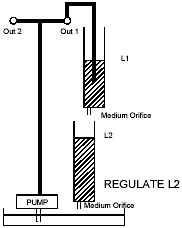
\includegraphics{images/1_relatorio/config_2.png}
    \caption{Sistema de tanques Acoplados}
    \label{fig:sistema_de_tanques_acoplados}
\end{figure}

%\newpage
%\cite{scilab2010}   
 
 
% tem que explicar o que é  sistema dinâmico de tanques acoplados: explicado (copiado do roteiro)
% software SCILAB/Xcos explicado

\end{flushleft}

\newpage

%%%%%%%%%% REFERENCIAL TEÓRICO %%%%%%%

\thispagestyle{main}

\section{REFERENCIAL TEÓRICO}


\subsection{Controladores PID e Sistemas Dinâmicos de Primeira Ordem}
%\subsection{Sistemas de Primeira Ordem}\hspace{4ex}

\hspace{4ex}O controlador PID, na realidade, pode ser visto como sendo uma família de controladores. As 3 ações de controle podem ser combinadas de diferentes maneiras, formando controladores que podem receber diferentes nomes, como: P, PI, PD, PID, conforme as ações de controle são, ou não, utilizadas.

\begin{enumerate}
    \item Controle Proporcional (P):
    \[u(t)=Kpe(t)\] 
    \[U(S)=KpE(S)\]
        \begin{itemize}
            \item O controlador proporcional é um amplificador, com ganho ajustável (K);
            \item O aumento do ganho K, diminui o erro de regime;
            \item Em geral, o aumento de K torna o sistema mais oscilatório, podendo instabilizá-lo;
            \item Melhora o regime e piora o transitório, sendo bastante limitado.
        \end{itemize}
        
    \item Controle Proporcional + Integral (PI):
    \[u(t)=Kp(e(t)+\frac{1}{\tau i}\int_{0}^{t}e(\tau)d\tau)\]
    \[U(S)=\frac{(KpS+Ki)}{s}E(s)\]
        \begin{itemize}
            \item A ação integral do controlador move a variável de controle C(S) baseada na integral no tempo do erro, sendo: \[Ki=\frac{Kp}{\tau i}\], em que: \[\tau i\] é o tempo integrativo, ou tempo de \emph{reset}, com unidade da ordem de minutos;
            \item Zera o erro de regime, pois aumenta o tipo do sistema em 1 unidade;
            \item É utilizado quanto tempos resposta transitória aceitável e resposta em regime insatisfatória;
            \item Adiciona um pólo em p=0 e um zero em \[z=\frac{ki}{kp}=\frac{-1}{\tau i}\]
            \item Como aumenta a ordem do sistema, temos possibilidade de instabilidade diferente do sistema original. Pode degradar o desempenho do controlador em malha fechada.
        \end{itemize}
        
    \item Controle Proporcional + Derivativo (PD):
        \[u(t)=Kp(e(t)+\tau d\frac{de(t)}{dt})\]
        \[U(S)=(Kp+KdS)E(S)\]
        \begin{itemize}
            \item Sendo: \[Kd=Kp\tau d\] a constante derivativa, dada em minutos.
            \item Leva em conta a taxa de variaçao do erro;
            \item É utilizado quando temos resposta em regime aceitável e resposta transitória insatisfatória;
            \item Adiciona um zero em \[z=\frac{-Kp}{Kd}=\frac{-1}{\tau d}\]
            \item Introduz um efeito de antecipação no sistema, fazendo com que o mesmo reaja não somente à magnitude do sinal de erro, como também à sua tendência para o instante futuro, iniciando, assim, uma ação corretiva mais cedo;
            \item A ação derivativa tem a desvantagem de amplificar os sinais de ruído, o que pode causar um efeito de saturação nos atuadores do sistema.
        \end{itemize}
        
    \item Controle Proporcional + Integral + Derivativo (PID):
        \[u(t)=Kp(e(t)+\frac{1}{\tau i}\int_{0}^{t}e(\tau)d(\tau)+\tau d\frac{de(t)}{dt})\]
        \[U(S)=(Kp+\frac{Ki}{s}+KdS)E(S) => \frac{U(S)}{E(S)}=\frac{KdS^2+KpS+Ki}{S}\]
        \begin{itemize}
                    \item É utilizado quando temos resposta transitória e em regime insatisfatórias simultaneamente;
            \item Adiciona um pólo em p=0 e 2 zeros, que dependem dos parâmetros do controlador.
        \end{itemize}
        
    \item Implementação do Controlador PID:
        \begin{itemize}
            \item Diferentes equipamentos, de diferentes fabricantes, podem apresentar pequenas variações quanto à implementação do controlador PID. As duas implementações mais comumente utilizadas são: \textbf{Ideal} e \textbf{Paralelo}.
        \end{itemize}
        
    \item Modificações das Ações de Controle PID:
        \begin{itemize}
            \item Existem também diversas modificações, que poderão ser necessárias em cada implementação, dependendo de características do sistema que estiver sendo controlado, das condições de operações as quais o sistema será submetido e, até mesmo, do equipamento que será utilizado para implementação do controlador.
        \end{itemize}
        
        \begin{enumerate}
            \item Modificação na Ação Derivativa:
                \begin{itemize}
                    \item Filtro da Ação Derivativa
                        \begin{figure}[h]
                            \centering
                            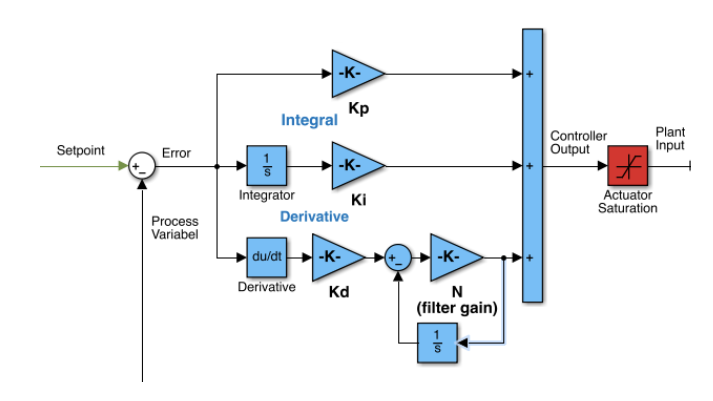
\includegraphics[width=15cm]{images/roteiro a/img ref teorico/filtro_de_acao_derivativa.png}
                            \caption{Filtro de Ação derivativa}
                            \label{fig:filtro_de_acao_derivativa}
                        \end{figure}
                    \item PI-D
                        \begin{figure}[h]
                            \centering
                            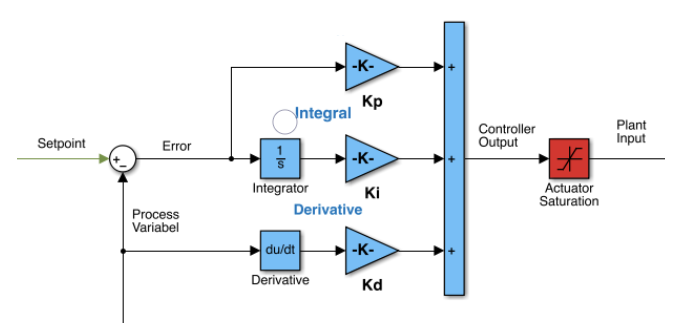
\includegraphics[width=15cm]{images/roteiro a/img ref teorico/pid.png}
                            \caption{PI-D}
                            \label{fig:pid}
                        \end{figure}
                        \begin{itemize}
                            \item Objetivo: Não derivar variações bruscas no sinal de referência. 
                        \end{itemize}
                        \newpage
                    \item I-PD
                         \begin{figure}[h]
                            \centering
                            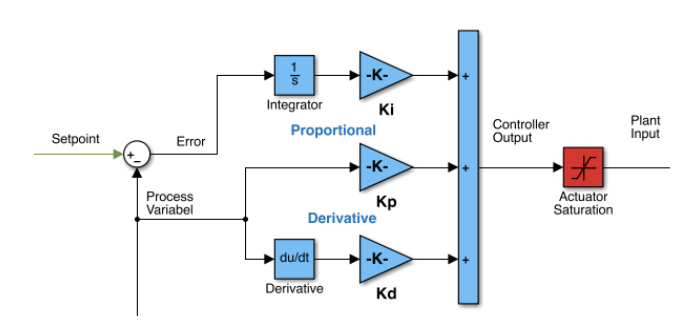
\includegraphics[width=15cm]{images/roteiro a/img ref teorico/ipd.png}
                            \caption{I-PD}
                            \label{fig:ipd}
                        \end{figure}
                        \begin{itemize}
                            \item Objetivo: Não derivar, nem amplificar variações bruscas no sinal de referência. 
                            \\
                        \end{itemize}
                \end{itemize} 
            \item Modificação na Ação Integrativa:
                \begin{itemize}
                    \item Filtro Anti-Windup (Anti-Reset Windup)
                \end{itemize}
                    \begin{figure}[h]
                            \centering
                            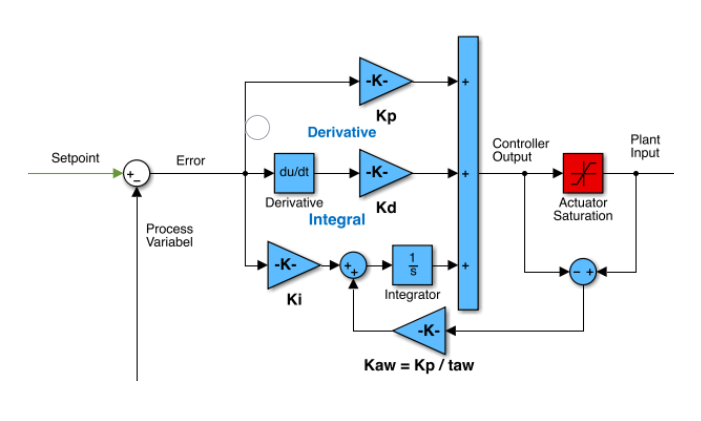
\includegraphics[width=15cm]{images/roteiro a/img ref teorico/filtro_anti_windup.png}
                            \caption{Filtro Anti-Windup (Anti-Reset Windup)}
                            \label{fig:filtro_anti_windup}
                        \end{figure}
        \end{enumerate}
\end{enumerate}
\newpage

\subsection{Sistemas de Segunda Ordem}
\hspace{4ex}Considere a seguinte equação diferencial de segunda ordem:
    \[a\frac{d^2e(t)}{dt^2}+b\frac{de(t)}{dt}+dc(t)=er(t)\]
Definindo:
    \[\frac{b}{a}=2\epsilon\omega_n; \hspace{4ex} \frac{d}{a}=\omega^2_n; \hspace{4ex} \frac{e}{a}=K;\]
onde \[\epsilon\] é o fator de amortecimento, \[\omega_n\] é a frequência natural e K é o ganho do sistema, temos:


\subsection{Sistemas de Segurança Instrumentados ou Intertravamentos}\hspace{4ex}

\subsection{Sistemas Dinâmicos na Configuração de Controle em Cascata}\hspace{4ex}

\newpage

%%%%%%%%%% METODOLOGIA %%%%%%%%%%%%%%%

\thispagestyle{main}

\section{METODOLOGIA}\hspace{4ex}
de fato escrever alguma coisa, como foi feita a simulação
\newpage

%%%%%%%%%% RESULTADOS %%%%%%%%%%%%%%%


\thispagestyle{main}

\section{RESULTADOS e DISCUSSÕES}\hspace{4ex}
%
%
Primeiramente, houveram testes de controle de primeira ordem, para entrada constante de valor 15 e senoidal,
$f(t)= 2sen(t)+10$

Depois, testes de controle de segunda ordem, para entrada constante de valor 15 e senoidal, de amplitude 2, bias 10 e frequência de 0.2 rad/s. Foram implementados intertravamentos para evitar transbordamento dos tanques ou succionar água (tensão negativa) quando o nível do primeiro tanque estiver muito baixo ou desligar (\emph{shutdown}) o sistema caso haja uma ocorrência anormal.

Testes de primeira e segunda ordem (sistemas 1 e 2) foram agrupados e discutidos em conjunto.

Por fim foram realizados testes com o controlador em cascata (mestre-escravo) e foi discutido como este tipo de configuração influencia no desempenho do sistema, em comparação ao sistemas de tipo 2 discutido anteriormente.
%
%
% 
% 
% 
\subsection{Controlador P}\hspace{4ex}

\begin{figure}[h]
    \foreach \kpSystemOne/\kpSystemTwo in {5/10,10/20,20/100}{
        \labABSubFigure{1}{P}{kp_\kpSystemOne}{K_p=\kpSystemOne}%1-1
        \labABSubFigure{2}{P}{kp_\kpSystemTwo}{K_p=\kpSystemTwo}%2-1
  }
\end{figure}

\hspace{4ex}
Testes de controle de primeira ordem, para entrada constante de valor 15 e senoidal, de amplitude 2 e bias 10.

Pode-se observar que, no sistema de tipo 1, com o aumento do ganho proporcional houve um
aumento na velocidade do sistema até a resposta em regime permanente e
uma diminuição do erro estacionário, ou seja,
a diferença entre a resposta desejada e a resposta em regime permanente. No senoidal ocorreu o mesmo, aumentando $K_p$ o nível do tanque 1 passa a seguir a referência e o nível do segundo passa a orbitar o bias, sem nunca estabilizar por causa da baixa frequência.

Observou-se que também que, no sistema de tipo 2,
o aumento de $K_p$ aumentou a oscilação do sistema mas diminuiu o 
erro de regime, não zerando-o completamente, como esperado. Sendo assim,
o sistema é do tipo subamortecido (0 < $\epsilon$ < 1), e considerando
que $K_p$ = $\omega_n^2$, a frequência aumenta com o ganho. Houve aumento
no tempo de acomodação e haveria também aumento significativo no
\emph{overshoot}, como se pode observar pela resposta do controlador
que é quase uma onda quadrada em $K_p$ = 100.
Não ocorreu devido a saturação do sistema. Com entrada senoidal, o aumento do $K_p$ resultou na resposta do segundo tanque seguir exatamente a referência e oscilações no nível do primeiro tanque.


\newpage

\subsection{Controlador PI}\hspace{4ex}
\begin{figure}[h]
    \foreach \kiSystemOne/\kiSystemTwo in {0.5/0.01,5/0.5,10/0.005}{
        \labABSubFigure{1}{PI}{kp_20_ki_\kiSystemOne}{K_p=20 \quad K_i=\kiSystemOne}%1-1
        \labABSubFigure{2}{PI}{kp_20_ki_\kiSystemTwo}{K_p=20 \quad K_i=\kiSystemTwo}%2-1
    }

\end{figure}

\hspace{4ex}


No sistema tipo 1, com a adição do controlador integral o sistema passa a ter comportamento de segunda ordem, subamortecido no exemplo, zerando o erro de regime observado anteriormente. No entanto, há bastante oscilação e o sistema é mais lento, chegando ao regime permanente em cerca de 3 vezes o tempo de sua contraparte apenas proporcional. Também há o custo do \emph{overshoot} de aproximadamente 36\% quando $K_i$ = 10, como observado. Para entrada senoidal o \emph{overshoot} também cresce com o aumento de $K_i$.

No sistema tipo 2, o erro de regime é automaticamente zerado, no entanto o intertravamento precisa agir mesmo para valores diminutos do ganho integral $K_i$ em 0.5, para que o tanque 1 não transborde (passe do nível 29). O efeito cumulativo da parcela integral do controlador, quando tem seu ganho aumentado, gera uma resposta mais oscilatória e com maior \emph{overshoot}, até que instabiliza o sistema em $K_i$ muito altos. Nesta situação o sistema continua a oscilar sem nunca chegar ao regime permanente em tempo plausível. Essa tendencia foi observada no experimento. Para entrada senoidal, o aumento de $K_i$ elevou o \emph{overshoot} do nível do segundo tanque e a oscilação do nível do primeiro, como esperado.


\newpage

\subsection{Controlador PD}\hspace{4ex}

\begin{figure}[h]
    \foreach \kdSystemOne/\kdSystemTwo in {1/1,5/15,15/25}{
        \labABSubFigure{1}{PD}{kp_20_kd_\kdSystemOne}{K_p=20 \quad K_d=\kdSystemOne}%1-1
        \labABSubFigure{2}{PD}{kp_20_kd_\kdSystemTwo}{K_p=20 \quad K_d=\kdSystemTwo}%2-1
    }
\end{figure}

\hspace{4ex}
Escrever sobre o Controlador PD

\newpage

\subsection{Controlador PID}\hspace{4ex}
\begin{figure}[h]
    \foreach \kiSystemOne/\kdSystemOne/\kiSystemTwo/\kdSystemTwo in {0.5/22/1/250,1/22/1/500,2/22/1/1000}{
        \labABSubFigure{1}{PID}{kp_20_ki_\kiSystemOne_kd_\kdSystemOne}
        {K_p=20 \quad K_i=\kiSystemOne \quad K_d=\kdSystemOne}%1-1
%
        \labABSubFigure{2}{PID}{kp_20_ki_\kiSystemTwo_kd_\kdSystemTwo}
        {K_p=20 \quad K_i=\kiSystemTwo \quad K_d=\kdSystemTwo}%2-1
    }
\end{figure}

\hspace{4ex}

Nesse contexto, o controlador proporcional ajusta a variável de controle proporcionalmente ao erro, o integral ajusta proporcional ao erro acumulado e a derivativa proporcional a velocidade de variação do erro. Permite um maior controle do comportamento do sistema, em relação aos anteriores. Observou-se um aumento no \emph{overshoot} ao se aumentar $K_i$ e uma maior oscilação com aumento de $K_p$.

Como observado no controlador PI, instabilização ocorre para maiores valores de $K_i$, onde o sistema nunca alcança regime permanente. O mesmo efeito ocorre ao se alterar $K_p$ mas não na mesma proporção. Alterar $K_d$ afeta notavelmente o tempo de acomodação e a sensibilidade do controlador ao efeito do ruído, como visto no do tipo PD. Para valores menores de $K_d$ (notadamente $K_d$ = 100) a frequência diminui de tal maneira a aumentar o tempo de acomodação. Para entrada senoidal, foi possível ajustar $K_i$ e $K_d$ para mitigar os efeitos de oscilação no nível do primeiro tanque ao mesmo tempo que se reduz a velocidade de regime transitório. 



\newpage

\subsection{Controlador PID com filtro na ação derivativa}\hspace{4ex}

\def \PIDDerivativeFilter{PID filtro derivativo}

\begin{figure}[h]
    \foreach \knSystemOne/\knSystemTwo in {0.5/30,50/50,100/100}{
        \labABSubFigure{1}{\PIDDerivativeFilter}
        {kp_20_ki_1_kd_1_kn_\knSystemOne}
        {K_p=20 \quad K_i=1 \quad K_d=1 \quad K_n=\knSystemOne}%1-1
%
        \labABSubFigure{2}{\PIDDerivativeFilter}
        {kp_20_ki_1_kd_1_kn_\knSystemTwo}
        {K_p=20 \quad K_i=1 \quad K_d=1 \quad K_n=\knSystemTwo}%2-1
  }
\end{figure}

\hspace{4ex}
Escrever sobre o Controlador PID com filtro na ação derivativa

\newpage

\subsection{Controlador PID com filtro anti-reset-windup}

\def \PIDFilter{PID filtro windup}

\begin{figure}[h]
\labABSubFigure{1}{\PIDFilter}{kp_0_5_ki_0_5_kd_0_05_kaw_0_5}{K_p=0.5 \quad K_i=0.5 \quad K_d=0.05 \quad K_{aw}=0.5}%1-1
\labABSubFigure{2}{\PIDFilter}{kp_20_ki_1_kd_1_kaw_1}{K_p=20 \quad K_i=1 \quad K_d=1 \quad K_{aw}=1}%2-1
\labABSubFigure{1}{\PIDFilter}{kp_0_5_ki_0_5_kd_0_05_kaw_1}{K_p=0.5 \quad K_i=0.5 \quad K_d=0.05 \quad K_{aw}=1}%1-2
\labABSubFigure{2}{\PIDFilter}{kp_20_ki_1_kd_20_kaw_1}{K_p=20 \quad K_i=1 \quad K_d=20 \quad K_{aw}=1}%2-2
\labABSubFigure{1}{\PIDFilter}{kp_0_5_ki_1_kd_0_05_kaw_0_5}{K_p=0.5 \quad K_i=1 \quad K_d=0.05 \quad K_{aw}=0.5}%1-3
\labABSubFigure{2}{\PIDFilter}{kp_20_ki_5_kd_1_kaw_1}{K_p=20 \quad K_i=5 \quad K_d=1 \quad K_{aw}=1}%2-3
\end{figure}

\hspace{4ex}
Quando o sistema está sujeito a um erro constante diferente de zero, o controlador integral tende a acumular seu efeito e requisitar comandos cada vez maiores ao atuador, mesmo estando saturado. Quando o erro eventualmente decresce e se torna negativo, há um tempo até que a saída integral “retorne” ao seu estado funcional, é o que se chama de tempo de \emph{windup}. O filtro \emph{anti-windup} contrabalanceia esse efeito somando ou subtraindo um valor proporcional ao ganho $K_aw$ quando há saturação (saída do controlador e entrada da planta são diferentes).

No primeiro sistema, o filtro \emph{anti-windup} atenua o efeito da parcela integral do controlador. Com $K_aw$ = 1 há uma leve redução do \emph{overshoot} e do tempo de acomodação. A frequência natural não foi modificada ao aumentar $K_aw$, apenas a mesma redução citada anteriormente, \emph{overshoot} por exemplo cai de 12\% para 9\%  aumentando o ganho do filtro de $K_aw$ 0.5 para 1. O \emph{overshoot} do tanque 2 é completamente removido para valores menores de $K_i$. Para entrada senoidal, o aumento de $K_aw$ 0.001 para 0.01 deslocou o bias dos níveis em -0.5, aproximadamente.

No segundo sistema, mesmo com $K_i$ = 1 a oscilação é controlada até que se aumente seu valor para algo mais considerável (no caso 5), onde há \emph{overshoot}. Aumentar $K_d$ tem efeito de redução da amplitude das oscilações, como esperado. Com entrada senoidal 


% 
% 
% 
% 
\subsection{Sistema de Controle Mestre-Escravo: Mestre P}

\subsubsection{Controlador Escravo P}
\begin{figure}[h]
\foreach \kp in {40,300,500}{
 \labMasterSlaveSubFigure{P}{P}{kp_master_\kp_kp_slave_\kp}
    {K_{p_{\textrm{mestre}}}=\kp \quad K_{p_{\textrm{escravo}}}=\kp }%
}
\end{figure}

Podemos Observar que quando maior o valor de $K_p$ mais próximo o nível do tanque se aproxíma da referência, também foi observado que a partir de 300
aumentar o seu valor deixa de surgir efeito. Resultados semelhetes encontrado com um controlador P, mas  diferente do controlador P, foi observado que é possível
controlar a variação do tanque 1, onde para valores baixos de  $K_{p_{\textrm{Escravo}}}$ a variação do nível do tanque 1 é baixa analogamente, valores altos aumenta a variação
do nível 1.

\newpage

\subsubsection{Controlador Escravo PD}

\begin{figure}[h]
\foreach \kdSlave in {100,1000,1000}{
    \labMasterSlaveSubFigure{P}{PD}{Kp_master_500_Kp_slave_500_Kd_slave_\kdSlave}
    {K_{p_{\textrm{mestre}}}=500 \quad K_{p_{\textrm{escravo}}}=500%
    \quad K_{d_{\textrm{escravo}}}=\kdSlave}%
    }
\end{figure}

Escrever sobre o Controlador PD

\newpage

\subsubsection{Controlador Escravo PI}

\begin{figure}[h]
\foreach \kiSlave in {3,6,12}{
    \labMasterSlaveSubFigure{P}{PI}{Kp_master_500_Kp_slave_500_Ki_slave_\kiSlave}
    {K_{p_{\textrm{mestre}}}=500 \quad K_{p_{\textrm{escravo}}}=500%
    \quad K_{i_{\textrm{escravo}}}=\kiSlave}%
    }
\end{figure}

Escrever sobre o Controlador PI

\newpage


\subsubsection{Controlador Escravo PID}

\begin{figure}[h]
    \foreach \ki/\kd in {0.5/5000,1/300,3/300}{
    \labMasterSlaveSubFigure{P}{PID}
    {Kp_master_500_Kp_slave_500_Ki_slave_\ki_Kd_slave_\kd}
    {K_{p_{\textrm{mestre}}}=500 \quad K_{p_{\textrm{escravo}}}=500%
    \quad K_{i_{\textrm{escravo}}}=\ki \quad K_{d_{\textrm{escravo}}}=\kd}%
    }
\end{figure}

Uma vez colocado o PID no Controlador escravo foi possível observar que apesar das constantes de controle influênciarem
fortemente no nível do tanque 1, é possível observar que essas influência alcança o nível 2, uma vez observado uma subida
sútil no gráfico a.

\newpage

\subsubsection{Controlador Escravo PID filtro derivativo}

\begin{figure}[h]
  \foreach \ki/\kd/\kn in {1/100/2,1/100/15,7/100/15}{
      \labMasterSlaveSubFigure{P}{PID filtro derivativo}
    {Kp_master_500_Kp_slave_500_Ki_slave_\ki_Kd_slave_\kd_Kn_slave_\kn}
    {K_{p_{\textrm{mestre}}}=500 \quad K_{p_{\textrm{escravo}}}=500%
    \quad K_{i_{\textrm{escravo}}}=\ki \quad K_{d_{\textrm{escravo}}}=\kd%
    \quad K_{n_{\textrm{escravo}}}=\kn }
    }
\end{figure}

Escrever sobre o Controlador PID com filtro na ação derivativa

\newpage

\subsubsection{Controlador Escravo PID filtro windup}

\begin{figure}[h]
  \foreach \ki/\kd/\kaw in {100/100/1,300/100/2,2000/100/3}{
      \labMasterSlaveSubFigure{P}{PID filtro windup}
    {Kp_master_500_Kp_slave_500_Ki_slave_\ki_Kd_slave_\kd_Kaw_slave_\kaw}
    {K_{p_{\textrm{mestre}}}=500 \quad K_{p_{\textrm{escravo}}}=500%
    \quad K_{i_{\textrm{escravo}}}=\ki \quad K_{d_{\textrm{escravo}}}=\kd%
    \quad K_{aw_{\textrm{escravo}}}=\kaw }
    }
\end{figure}
%
O controlador Escravo PID com o Windup, permite diminuir o overshooting, a variação do nível 1 e o tempo de decida
do nível do tanque 1 sem precisar aumentar as constantes derivativas.
% 
% 
\newpage
%
% 
\subsection{Sistema de Controle Mestre-Escravo: Mestre PD}
%
\def \currentMaster{Mestre PD}
\def \currentSlave{escravo P}
\def \masterSlaveCaption{ \currentMaster - \currentSlave }
%
\def \controllerPEvaluation{resultados/roteiro_c/mestre_PD/Controlador_P}
\def \controllerPDEvaluation{resultados/roteiro_c/mestre_PD/Controlador_PD}
\def \controllerPIEvaluation{resultados/roteiro_c/mestre_PD/Controlador_PI}
\def \controllerPIDEvaluation{resultados/roteiro_c/mestre_PD/Controlador_PID}
\def \controllerPIDDevvaluation{resultados/roteiro_c/mestre_PD/Controlador_PID_filtro_dev}
\def \controllerPIDWindupEvaluation{resultados/roteiro_c/mestre_PD/Controlador_PID_filtro_windup}
%
%
\subsubsection{Controlador Escravo P}
\begin{figure}[h]
\foreach \kd in {500,1000,10000}{ %kp_master_500_kd_master_500_kp_slave_500
 \labMasterSlaveSubFigure{PD}{P}{kp_master_500_kd_master_\kd_kp_slave_500}
    {K_{p_{\textrm{mestre}}}=500 \quad K_{d_{\textrm{mestre}}}=\kd \quad K_{p_{\textrm{escravo}}}=500 }%
}
\controllerCaption{1}{\masterSlaveCaption}
\end{figure}

\input{\controllerPEvaluation}

\newpage
%
\def \currentSlave{escravo PD}
%
\subsubsection{Controlador Escravo PD}

\begin{figure}[h]
\foreach \kdMaster/\kdSlave in {1/1,1/100,5/100}{
    \labMasterSlaveSubFigure{PD}{PD}
    {Kp_master_500_Kd_master_\kdMaster_Kp_slave_500_Kd_slave_\kdSlave}
    {K_{p_{\textrm{mestre}}}=500 \quad K_{d_{\textrm{mestre}}}=\kdMaster
    \quad K_{p_{\textrm{escravo}}}=500 \quad K_{d_{\textrm{escravo}}}=\kdSlave}%
    }
    \controllerCaption{1}{\masterSlaveCaption}
\end{figure}

\input{\controllerPDEvaluation}

\newpage
%
\def \currentSlave{escravo PI}
%

\subsubsection{Controlador Escravo PI}

\begin{figure}[h]
\foreach \kdMaster/\kiSlave in {1/10,1/50,10000/10}{
    \labMasterSlaveSubFigure{PD}{PI}
    {Kp_master_500_Kd_master_\kdMaster_Kp_slave_500_Ki_slave_\kiSlave}
    {K_{p_{\textrm{mestre}}}=500 \quad K_{d_{\textrm{mestre}}}=\kdMaster \quad K_{p_{\textrm{escravo}}}=500 \quad K_{i_{\textrm{escravo}}}=\kiSlave}%
    }
    \controllerCaption{1}{\masterSlaveCaption}
\end{figure}

\input{\controllerPIEvaluation}

\newpage
%
\def \currentSlave{escravo PID}
%


\subsubsection{Controlador Escravo PID}

\begin{figure}[h]
\foreach  \kdMaster/\kiSlave/\kdSlave in {1/10/500,1/20/2000,2/20/2000}{
\labMasterSlaveSubFigure{PD}{PID}
{Kp_master_500_Kd_master_\kdMaster_kp_slave_500_ki_slave_\kiSlave_kd_slave_\kdSlave}
{K_{p_{\textrm{mestre}}}=500 \quad K_{d_{\textrm{mestre}}}=\kdMaster \quad K_{p_{\textrm{escravo}}}=500 \quad K_{i_{\textrm{escravo}}}=\kiSlave \quad K_{d_{\textrm{escravo}}}=\kdSlave}
}
\controllerCaption{1}{\masterSlaveCaption}
\end{figure}

\input{\controllerPIDEvaluation}

\newpage
%
\def \currentSlave{escravo PID filtro derivativo}
%
\subsubsection{Controlador Escravo PID filtro derivativo}

\begin{figure}[h]
  \foreach \kdMaster/\ki/\kd/\kn in {1/20/2000/1.5,2/20/2000/1.5,2/20/2500/0.75}{
      \labMasterSlaveSubFigure{PD}{PID filtro derivativo}
    {Kp_master_500_Kd_master_\kdMaster_Kp_slave_500_Ki_slave_\ki_Kd_slave_\kd_Kn_slave_\kn}
    {K_{p_{\textrm{mestre}}}=500 \quad K_{d_{\textrm{master}}}=\kdMaster%
    K_{p_{\textrm{escravo}}}=500 \quad K_{i_{\textrm{escravo}}}=\ki%
    \quad K_{d_{\textrm{escravo}}}=\kd \quad K_{n_{\textrm{escravo}}}=\kn}
    }
    \controllerCaption{1}{\masterSlaveCaption}
\end{figure}
\input{\controllerPIDDevvaluation}

\newpage
%
\def \currentSlave{escravo PID filtro windup}
%
\subsubsection{Controlador Escravo PID filtro windup}

\begin{figure}[h]
  \foreach \kdMaster/\ki/\kd/\kaw in {1/10/2/0.005,2.5/50/2.5/0.01,3/50/3/0.15}{
      \labMasterSlaveSubFigure{PD}{PID filtro windup}
    {Kp_master_500_Kd_master_\kdMaster_Kp_slave_500_Ki_slave_\ki_Kd_slave_\kd_Kaw_slave_\kaw}
    {K_{p_{\textrm{mestre}}}=500 \quad K_{d_{\textrm{mestre}}}=\kdMaster \quad %
     K_{p_{\textrm{escravo}}}=500 \quad K_{i_{\textrm{escravo}}}=\ki \quad  %
    K_{d_{\textrm{escravo}}}=\kd \quad K_{aw_{\textrm{escravo}}}=\kaw }
    }
    \controllerCaption{1}{\masterSlaveCaption}
\end{figure}

\input{\controllerPIDWindupEvaluation}

\newpage
%
% 
\subsection{Sistema de Controle Mestre-Escravo: Mestre PI
}
%
\def \currentMaster{PI}
\def \currentSlave{escravo P}
\def \masterSlaveCaption{Mestre \currentMaster - \currentSlave }
\def \rootDir{mestre_PI}
%
\def \controllerPEvaluation{resultados/roteiro_c/\rootDir/Controlador_P}
\def \controllerPDEvaluation{resultados/roteiro_c/\rootDir/Controlador_PD}
\def \controllerPIEvaluation{resultados/roteiro_c/\rootDir/Controlador_PI}
\def \controllerPIDEvaluation{resultados/roteiro_c/\rootDir/Controlador_PID}
\def \controllerPIDDevvaluation{resultados/roteiro_c/\rootDir/Controlador_PID_filtro_dev}
\def \controllerPIDWindupEvaluation{resultados/roteiro_c/\rootDir/Controlador_PID_filtro_windup}
%
%
%
%
\subsubsection{Controlador Escravo P}
\begin{figure}[h]
    \labMasterSlaveSubFigure{PI}
{P}
{Kp_master_500_Ki_master_2_Kp_slave_500}
{K_{p_{\textrm{mestre}}}=500 \quad K_{i_{\textrm{mestre}}}=2 \quad K_{p_{\textrm{escravo}}}=500}
\labMasterSlaveSubFigure{PI}
{P}
{Kp_master_500_Ki_master_20_Kp_slave_500}
{K_{p_{\textrm{mestre}}}=500 \quad K_{i_{\textrm{mestre}}}=20 \quad K_{p_{\textrm{escravo}}}=500}
\labMasterSlaveSubFigure{PI}
{P}
{Kp_master_500_Ki_master_50_Kp_slave_500}
{K_{p_{\textrm{mestre}}}=500 \quad K_{i_{\textrm{mestre}}}=50 \quad K_{p_{\textrm{escravo}}}=500}

    \controllerCaption{1}{\masterSlaveCaption}
\end{figure}

\input{\controllerPEvaluation}

\newpage
%
\def \currentSlave{escravo PD}
%
\subsubsection{Controlador Escravo PD}

\begin{figure}[h]
    \labMasterSlaveSubFigure{PI}
{PD}
{Kp_master_500_Ki_master_0_5_Kp_slave_500_Kd_slave_10000}
{K_{p_{\textrm{mestre}}}=500 \quad K_{i_{\textrm{mestre}}}=0.5 \quad K_{p_{\textrm{escravo}}}=500 \quad K_{d_{\textrm{escravo}}}=10000}
\labMasterSlaveSubFigure{PI}
{PD}
{Kp_master_500_Ki_master_0_5_Kp_slave_500_Kd_slave_1000}
{K_{p_{\textrm{mestre}}}=500 \quad K_{i_{\textrm{mestre}}}=0.5 \quad K_{p_{\textrm{escravo}}}=500 \quad K_{d_{\textrm{escravo}}}=1000}
\labMasterSlaveSubFigure{PI}
{PD}
{Kp_master_500_Ki_master_2_Kp_slave_500_Kd_slave_300}
{K_{p_{\textrm{mestre}}}=500 \quad K_{i_{\textrm{mestre}}}=2 \quad K_{p_{\textrm{escravo}}}=500 \quad K_{d_{\textrm{escravo}}}=300}

    \controllerCaption{1}{\masterSlaveCaption}
\end{figure}

\input{\controllerPDEvaluation}

\newpage
%
\def \currentSlave{escravo PI}
%

\subsubsection{Controlador Escravo PI}

\begin{figure}[h]
    \labMasterSlaveSubFigure{PI}
{PI}
{Kp_master_500_Ki_master_0_5_Kp_slave_500_Ki_slave_0_5}
{K_{p_{\textrm{mestre}}}=500 \quad K_{i_{\textrm{mestre}}}=0.5 \quad K_{p_{\textrm{escravo}}}=500 \quad K_{i_{\textrm{escravo}}}=0.5}
\labMasterSlaveSubFigure{PI}
{PI}
{Kp_master_500_Ki_master_0_5_Kp_slave_500_Ki_slave_1}
{K_{p_{\textrm{mestre}}}=500 \quad K_{i_{\textrm{mestre}}}=0.5 \quad K_{p_{\textrm{escravo}}}=500 \quad K_{i_{\textrm{escravo}}}=1}
\labMasterSlaveSubFigure{PI}
{PI}
{Kp_master_500_Ki_master_0_5_Kp_slave_500_Ki_slave_5}
{K_{p_{\textrm{mestre}}}=500 \quad K_{i_{\textrm{mestre}}}=0.5 \quad K_{p_{\textrm{escravo}}}=500 \quad K_{i_{\textrm{escravo}}}=5}

    \controllerCaption{1}{\masterSlaveCaption}
\end{figure}

\input{\controllerPIEvaluation}

\newpage
%
\def \currentSlave{escravo PID}
%


\subsubsection{Controlador Escravo PID}

\begin{figure}[h]
    \labMasterSlaveSubFigure{PI}
{PID}
{Kp_master_500_Ki_master_0_5_Kp_slave_500_Ki_slave_0_5_Kd_slave_10000}
{K_{p_{\textrm{mestre}}}=500 \quad K_{i_{\textrm{mestre}}}=0.5 \quad K_{p_{\textrm{escravo}}}=500 \quad K_{i_{\textrm{escravo}}}=0.5 \quad K_{d_{\textrm{escravo}}}=10000}
\labMasterSlaveSubFigure{PI}
{PID}
{Kp_master_500_Ki_master_0_5_Kp_slave_500_Ki_slave_0_5_Kd_slave_1000}
{K_{p_{\textrm{mestre}}}=500 \quad K_{i_{\textrm{mestre}}}=0.5 \quad K_{p_{\textrm{escravo}}}=500 \quad K_{i_{\textrm{escravo}}}=0.5 \quad K_{d_{\textrm{escravo}}}=1000}
\labMasterSlaveSubFigure{PI}
{PID}
{Kp_master_500_Ki_master_0_5_Kp_slave_500_Ki_slave_0_5_Kd_slave_500}
{K_{p_{\textrm{mestre}}}=500 \quad K_{i_{\textrm{mestre}}}=0.5 \quad K_{p_{\textrm{escravo}}}=500 \quad K_{i_{\textrm{escravo}}}=0.5 \quad K_{d_{\textrm{escravo}}}=500}

    \controllerCaption{1}{\masterSlaveCaption}
\end{figure}

\input{\controllerPIDEvaluation}

\newpage
%
\def \currentSlave{escravo PID filtro derivativo}
%
\subsubsection{Controlador Escravo PID filtro derivativo}

\begin{figure}[h]
    \labMasterSlaveSubFigure{PI}
{PID filtro derivativo}
{Kp_master_500_Ki_master_2_Kp_slave_500_Ki_slave_0_5_Kd_slave_10000_Kn_slave_1}
{K_{p_{\textrm{mestre}}}=500 \quad K_{i_{\textrm{mestre}}}=2 \quad K_{p_{\textrm{escravo}}}=500 \quad K_{i_{\textrm{escravo}}}=0.5 \quad K_{d_{\textrm{escravo}}}=10000 \quad K_{n_{\textrm{escravo}}}=1}
\labMasterSlaveSubFigure{PI}
{PID filtro derivativo}
{Kp_master_500_Ki_master_2_Kp_slave_500_Ki_slave_0_5_Kd_slave_10000_Kn_slave_2}
{K_{p_{\textrm{mestre}}}=500 \quad K_{i_{\textrm{mestre}}}=2 \quad K_{p_{\textrm{escravo}}}=500 \quad K_{i_{\textrm{escravo}}}=0.5 \quad K_{d_{\textrm{escravo}}}=10000 \quad K_{n_{\textrm{escravo}}}=2}
\labMasterSlaveSubFigure{PI}
{PID filtro derivativo}
{Kp_master_500_Ki_master_30_Kp_slave_500_Ki_slave_0_5_Kd_slave_10000_Kn_slave_4_5}
{K_{p_{\textrm{mestre}}}=500 \quad K_{i_{\textrm{mestre}}}=30 \quad K_{p_{\textrm{escravo}}}=500 \quad K_{i_{\textrm{escravo}}}=0.5 \quad K_{d_{\textrm{escravo}}}=10000 \quad K_{n_{\textrm{escravo}}}=4.5}

    \controllerCaption{1}{\masterSlaveCaption}
\end{figure}
\input{\controllerPIDDevvaluation}

\newpage
%
\def \currentSlave{escravo PID filtro windup}
%
\subsubsection{Controlador Escravo PID filtro windup}

\begin{figure}[h]
    \labMasterSlaveSubFigure{PI}
{PID filtro windup}
{Kp_master_500_Ki_master_200_Kp_slave_500_Ki_slave_0_5_Kd_slave_45_Kaw_slave_2}
{K_{p_{\textrm{mestre}}}=500 \quad K_{i_{\textrm{mestre}}}=200 \quad K_{p_{\textrm{escravo}}}=500 \quad K_{i_{\textrm{escravo}}}=0.5 \quad K_{d_{\textrm{escravo}}}=45 \quad K_{aw_{\textrm{escravo}}}=2}
\labMasterSlaveSubFigure{PI}
{PID filtro windup}
{Kp_master_500_Ki_master_300_Kp_slave_500_Ki_slave_0_5_Kd_slave_45_Kaw_slave_2}
{K_{p_{\textrm{mestre}}}=500 \quad K_{i_{\textrm{mestre}}}=300 \quad K_{p_{\textrm{escravo}}}=500 \quad K_{i_{\textrm{escravo}}}=0.5 \quad K_{d_{\textrm{escravo}}}=45 \quad K_{aw_{\textrm{escravo}}}=2}
\labMasterSlaveSubFigure{PI}
{PID filtro windup}
{Kp_master_500_Ki_master_300_Kp_slave_500_Ki_slave_0_5_Kd_slave_45_Kaw_slave_5}
{K_{p_{\textrm{mestre}}}=500 \quad K_{i_{\textrm{mestre}}}=300 \quad K_{p_{\textrm{escravo}}}=500 \quad K_{i_{\textrm{escravo}}}=0.5 \quad K_{d_{\textrm{escravo}}}=45 \quad K_{aw_{\textrm{escravo}}}=5}

    \controllerCaption{1}{\masterSlaveCaption}
\end{figure}

\input{\controllerPIDWindupEvaluation}

\newpage
%
% 
\subsection{Sistema de Controle Mestre-Escravo: Mestre PID
}
%
\def \currentMaster{PID}
\def \currentSlave{escravo P}
\def \masterSlaveCaption{Mestre \currentMaster - \currentSlave }
\def \rootDir{mestre_PID}
%
\def \controllerPEvaluation{resultados/roteiro_c/\rootDir/Controlador_P}
\def \controllerPDEvaluation{resultados/roteiro_c/\rootDir/Controlador_PD}
\def \controllerPIEvaluation{resultados/roteiro_c/\rootDir/Controlador_PI}
\def \controllerPIDEvaluation{resultados/roteiro_c/\rootDir/Controlador_PID}
\def \controllerPIDDevvaluation{resultados/roteiro_c/\rootDir/Controlador_PID_filtro_dev}
\def \controllerPIDWindupEvaluation{resultados/roteiro_c/\rootDir/Controlador_PID_filtro_windup}
%
%
%
%
\subsubsection{Controlador Escravo P}
\begin{figure}[h]
    \labMasterSlaveSubFigure{PID}
{P}
{Kp_master_500_Ki_master_1_Kd_master_1_Kp_slave_500}
{K_{p_{\textrm{mestre}}}=500 \quad K_{i_{\textrm{mestre}}}=2 \quad K_{d_{\textrm{mestre}}}=1 \quad K_{p_{\textrm{escravo}}}=500}
\labMasterSlaveSubFigure{PID}
{P}
{Kp_master_500_Ki_master_1_Kd_master_500_Kp_slave_500}
{K_{p_{\textrm{mestre}}}=500 \quad K_{i_{\textrm{mestre}}}=1 \quad K_{d_{\textrm{mestre}}}=500 \quad K_{p_{\textrm{escravo}}}=500}
\labMasterSlaveSubFigure{PID}
{P}
{Kp_master_500_Ki_master_30_Kd_master_500_Kp_slave_500}
{K_{p_{\textrm{mestre}}}=500 \quad K_{i_{\textrm{mestre}}}=30 \quad K_{d_{\textrm{mestre}}}=500 \quad K_{p_{\textrm{escravo}}}=500}

    \controllerCaption{1}{\masterSlaveCaption}
\end{figure}

\input{\controllerPEvaluation}

\newpage
%
\def \currentSlave{escravo PD}
%
\subsubsection{Controlador Escravo PD}

\begin{figure}[h]
    \labMasterSlaveSubFigure{PID}
{PD}
{Kp_master_500_Ki_master_30_Kd_master_500_Kp_slave_500_Kd_slave_2}
{K_{p_{\textrm{mestre}}}=500 \quad K_{i_{\textrm{mestre}}}=30 \quad K_{d_{\textrm{mestre}}}=500 \quad K_{p_{\textrm{escravo}}}=500 \quad K_{d_{\textrm{escravo}}}=2}
\labMasterSlaveSubFigure{PID}
{PD}
{Kp_master_500_Ki_master_30_Kd_master_500_Kp_slave_500_Kd_slave_5}
{K_{p_{\textrm{mestre}}}=500 \quad K_{i_{\textrm{mestre}}}=30\quad K_{d_{\textrm{mestre}}}=500 \quad K_{p_{\textrm{escravo}}}=500 \quad K_{d_{\textrm{escravo}}}=5}
\labMasterSlaveSubFigure{PID}
{PD}
{Kp_master_500_Ki_master_30_Kd_master_500_Kp_slave_500_Kd_slave_10}
{K_{p_{\textrm{mestre}}}=500 \quad K_{i_{\textrm{mestre}}}=30 \quad K_{d_{\textrm{mestre}}}=500 \quad K_{p_{\textrm{escravo}}}=500 \quad K_{d_{\textrm{escravo}}}=10}

    \controllerCaption{1}{\masterSlaveCaption}
\end{figure}

\input{\controllerPDEvaluation}

\newpage
%
\def \currentSlave{escravo PI}
%

\subsubsection{Controlador Escravo PI}

\begin{figure}[h]
    \labMasterSlaveSubFigure{PID}
{PI}
{Kp_master_500_Ki_master_30_Kd_master_500_Kp_slave_500_Ki_slave_5}
{K_{p_{\textrm{mestre}}}=500 \quad K_{i_{\textrm{mestre}}}=30 \quad K_{d_{\textrm{mestre}}}=500 \quad K_{p_{\textrm{escravo}}}=500 \quad K_{i_{\textrm{escravo}}}=5}
\labMasterSlaveSubFigure{PID}
{PI}
{Kp_master_500_Ki_master_30_Kd_master_500_Kp_slave_500_Ki_slave_10}
{K_{p_{\textrm{mestre}}}=500 \quad K_{i_{\textrm{mestre}}}=30 \quad K_{d_{\textrm{mestre}}}=500 \quad K_{p_{\textrm{escravo}}}=500 \quad K_{i_{\textrm{escravo}}}=10}
\labMasterSlaveSubFigure{PID}
{PI}
{Kp_master_500_Ki_master_30_Kd_master_10000_Kp_slave_500_Ki_slave_0_5}
{K_{p_{\textrm{mestre}}}=500 \quad K_{i_{\textrm{mestre}}}=30 \quad K_{d_{\textrm{mestre}}}=10000 \quad K_{p_{\textrm{escravo}}}=500 \quad K_{i_{\textrm{escravo}}}=0.5}

    \controllerCaption{1}{\masterSlaveCaption}
\end{figure}

\input{\controllerPIEvaluation}

\newpage
%
\def \currentSlave{escravo PID}
%


\subsubsection{Controlador Escravo PID}

\begin{figure}[h]
    \labMasterSlaveSubFigure{PID}
{PID}
{Kp_master_500_Ki_master_30_Kd_master_500_Kp_slave_500_Ki_slave_0_5_Kd_slave_2}
{K_{p_{\textrm{mestre}}}=500 \quad K_{i_{\textrm{mestre}}}=30 \quad K_{d_{\textrm{mestre}}}=500 \quad K_{p_{\textrm{escravo}}}=500 \quad K_{i_{\textrm{escravo}}}=0.5 \quad K_{d_{\textrm{escravo}}}=2}
\labMasterSlaveSubFigure{PID}
{PID}
{Kp_master_500_Ki_master_30_Kd_master_500_Kp_slave_500_Ki_slave_0_5_Kd_slave_5}
{K_{p_{\textrm{mestre}}}=500 \quad K_{i_{\textrm{mestre}}}=30 \quad K_{d_{\textrm{mestre}}}=500 \quad K_{p_{\textrm{escravo}}}=500 \quad K_{i_{\textrm{escravo}}}=0.5 \quad K_{d_{\textrm{escravo}}}=5}
\labMasterSlaveSubFigure{PID}
{PID}
{Kp_master_500_Ki_master_30_Kd_master_10000_Kp_slave_500_Ki_slave_0_5_Kd_slave_1}
{K_{p_{\textrm{mestre}}}=500 \quad K_{i_{\textrm{mestre}}}=30 \quad K_{d_{\textrm{mestre}}}=10000 \quad K_{p_{\textrm{escravo}}}=500 \quad K_{i_{\textrm{escravo}}}=0.5 \quad K_{d_{\textrm{escravo}}}=1}

    \controllerCaption{1}{\masterSlaveCaption}
\end{figure}

\input{\controllerPIDEvaluation}

\newpage
%
\def \currentSlave{escravo PID filtro derivativo}
%
\subsubsection{Controlador Escravo PID filtro derivativo}

\begin{figure}[h]
    \labMasterSlaveSubFigure{PID}
{PID filtro derivativo}
{Kp_master_500_Ki_master_30_Kd_master_500_Kp_slave_500_Ki_slave_0_5_Kd_slave_5_Kn_slave_1}
{K_{p_{\textrm{mestre}}}=500 \quad K_{i_{\textrm{mestre}}}=30 \quad K_{d_{\textrm{mestre}}}=500 \quad K_{p_{\textrm{escravo}}}=500 \quad K_{i_{\textrm{escravo}}}=0.5 \quad K_{d_{\textrm{escravo}}}=10000 \quad K_{n_{\textrm{escravo}}}=1}
\labMasterSlaveSubFigure{PID}
{PID filtro derivativo}
{Kp_master_500_Ki_master_30_Kd_master_500_Kp_slave_500_Ki_slave_0_5_Kd_slave_5_Kn_slave_2}
{K_{p_{\textrm{mestre}}}=500 \quad K_{i_{\textrm{mestre}}}=30 \quad K_{d_{\textrm{mestre}}}=500 \quad K_{p_{\textrm{escravo}}}=500 \quad K_{i_{\textrm{escravo}}}=0.5 \quad K_{d_{\textrm{escravo}}}=10000 \quad K_{n_{\textrm{escravo}}}=2}
\labMasterSlaveSubFigure{PID}
{PID filtro derivativo}
{Kp_master_500_Ki_master_30_Kd_master_500_Kp_slave_500_Ki_slave_0_5_Kd_slave_5_Kn_slave_3}
{K_{p_{\textrm{mestre}}}=500 \quad K_{i_{\textrm{mestre}}}=30 \quad K_{d_{\textrm{mestre}}}=500 \quad K_{p_{\textrm{escravo}}}=500 \quad K_{i_{\textrm{escravo}}}=0.5 \quad K_{d_{\textrm{escravo}}}=10000 \quad K_{n_{\textrm{escravo}}}=3}

    \controllerCaption{1}{\masterSlaveCaption}
\end{figure}
\input{\controllerPIDDevvaluation}

\newpage
%
\def \currentSlave{escravo PID filtro windup}
%
\subsubsection{Controlador Escravo PID filtro windup}

\begin{figure}[h]
    \labMasterSlaveSubFigure{PID}
{PID filtro windup}
{Kp_master_500_Ki_master_5_Kd_master_500_Kp_slave_500_Ki_slave_5_Kd_slave_1_Kaw_slave_0_005}
{K_{p_{\textrm{mestre}}}=500 \quad K_{i_{\textrm{mestre}}}=5 \quad K_{d_{\textrm{mestre}}}=500 \quad K_{p_{\textrm{escravo}}}=500 \quad K_{i_{\textrm{escravo}}}=5 \quad K_{d_{\textrm{escravo}}}=1 \quad K_{aw_{\textrm{escravo}}}=0.005}
\labMasterSlaveSubFigure{PID}
{PID filtro windup}
{Kp_master_500_Ki_master_30_Kd_master_500_Kp_slave_500_Ki_slave_0_5_Kd_slave_5_Kaw_slave_0_005}
{K_{p_{\textrm{mestre}}}=500 \quad K_{i_{\textrm{mestre}}}=30 \quad K_{d_{\textrm{mestre}}}=500 \quad K_{p_{\textrm{escravo}}}=500 \quad K_{i_{\textrm{escravo}}}=0.5 \quad K_{d_{\textrm{escravo}}}=5 \quad K_{aw_{\textrm{escravo}}}=0.005}
\labMasterSlaveSubFigure{PID}
{PID filtro windup}
{Kp_master_500_Ki_master_30_Kd_master_500_Kp_slave_500_Ki_slave_30_Kd_slave_1_Kaw_slave_0_005}
{K_{p_{\textrm{mestre}}}=500 \quad K_{i_{\textrm{mestre}}}=30 \quad K_{d_{\textrm{mestre}}}=500 \quad K_{p_{\textrm{escravo}}}=500 \quad K_{i_{\textrm{escravo}}}=30 \quad K_{d_{\textrm{escravo}}}=1 \quad K_{aw_{\textrm{escravo}}}=0.005}

    \controllerCaption{1}{\masterSlaveCaption}
\end{figure}

\input{\controllerPIDWindupEvaluation}

\newpage
%
% 
\subsection{Sistema de Controle Mestre-Escravo: Mestre PID filtro derivativo
}
%
\def \currentMaster{PID filtro derivativo}
\def \currentSlave{escravo P}
\def \masterSlaveCaption{Mestre \currentMaster - \currentSlave }
\def \rootDir{mestre_PID_filtro_derivativo}
%
\def \controllerPEvaluation{resultados/roteiro_c/\rootDir/Controlador_P}
\def \controllerPDEvaluation{resultados/roteiro_c/\rootDir/Controlador_PD}
\def \controllerPIEvaluation{resultados/roteiro_c/\rootDir/Controlador_PI}
\def \controllerPIDEvaluation{resultados/roteiro_c/\rootDir/Controlador_PID}
\def \controllerPIDDevvaluation{resultados/roteiro_c/\rootDir/Controlador_PID_filtro_dev}
\def \controllerPIDWindupEvaluation{resultados/roteiro_c/\rootDir/Controlador_PID_filtro_windup}
%
%
%
%
\subsubsection{Controlador Escravo P}
\begin{figure}[h]
    \labMasterSlaveSubFigure{PID filtro derivativo}
{P}
{Kp_master_500_Ki_master_1_Kd_master_1_Kn_master_1_Kp_slave_500}
{K_{p_{\textrm{mestre}}}=500 \quad K_{i_{\textrm{mestre}}}=1 \quad K_{d_{\textrm{mestre}}}=1 \quad K_{n_{\textrm{mestre}}}=1 \quad K_{p_{\textrm{escravo}}}=500}
\labMasterSlaveSubFigure{PID filtro derivativo}
{P}
{Kp_master_500_Ki_master_7_Kd_master_1_Kn_master_200_Kp_slave_500}
{K_{p_{\textrm{mestre}}}=500 \quad K_{i_{\textrm{mestre}}}=7 \quad K_{d_{\textrm{mestre}}}=1 \quad K_{n_{\textrm{mestre}}}=200 \quad K_{p_{\textrm{escravo}}}=500}
\labMasterSlaveSubFigure{PID filtro derivativo}
{P}
{Kp_master_500_Ki_master_7_Kd_master_1_Kn_master_500_Kp_slave_500}
{K_{p_{\textrm{mestre}}}=500 \quad K_{i_{\textrm{mestre}}}=7 \quad K_{d_{\textrm{mestre}}}=1 \quad K_{n_{\textrm{mestre}}}=500 \quad K_{p_{\textrm{escravo}}}=500}

    \controllerCaption{1}{\masterSlaveCaption}
\end{figure}

\input{\controllerPEvaluation}

\newpage
%
\def \currentSlave{escravo PD}
%
\subsubsection{Controlador Escravo PD}

\begin{figure}[h]
    \labMasterSlaveSubFigure{PID filtro derivativo}
{PD}
{Kp_master_500_Ki_master_100_Kd_master_1_Kn_master_500_Kp_slave_500_Kd_slave_2}
{K_{p_{\textrm{mestre}}}=500 \quad K_{i_{\textrm{mestre}}}=100 \quad K_{d_{\textrm{mestre}}}=1 \quad K_{n_{\textrm{mestre}}}=500 \quad K_{p_{\textrm{escravo}}}=500 \quad K_{d_{\textrm{escravo}}}=2}
\labMasterSlaveSubFigure{PID filtro derivativo}
{PD}
{Kp_master_500_Ki_master_100_Kd_master_1_Kn_master_500_Kp_slave_500_Kd_slave_3}
{K_{p_{\textrm{mestre}}}=500 \quad K_{i_{\textrm{mestre}}}=100\quad K_{d_{\textrm{mestre}}}=1 \quad K_{n_{\textrm{mestre}}}=500 \quad K_{p_{\textrm{escravo}}}=500 \quad K_{d_{\textrm{escravo}}}=3}
\labMasterSlaveSubFigure{PID filtro derivativo}
{PD}
{Kp_master_500_Ki_master_100_Kd_master_1_Kn_master_500_Kp_slave_500_Kd_slave_5}
{K_{p_{\textrm{mestre}}}=500 \quad K_{i_{\textrm{mestre}}}=100 \quad K_{d_{\textrm{mestre}}}=1 \quad K_{n_{\textrm{mestre}}}=500 \quad K_{p_{\textrm{escravo}}}=500 \quad K_{d_{\textrm{escravo}}}=5}

    \controllerCaption{1}{\masterSlaveCaption}
\end{figure}

\input{\controllerPDEvaluation}

\newpage
%
\def \currentSlave{escravo PI}
%

\subsubsection{Controlador Escravo PI}

\begin{figure}[h]
    \labMasterSlaveSubFigure{PID filtro derivativo}
{PI}
{Kp_master_500_Ki_master_1_Kd_master_1_Kn_master_750_Kp_slave_500_Ki_slave_14}
{K_{p_{\textrm{mestre}}}=500 \quad K_{i_{\textrm{mestre}}}=1 \quad K_{d_{\textrm{mestre}}}=1 \quad K_{n_{\textrm{mestre}}}=750 \quad K_{p_{\textrm{escravo}}}=500 \quad K_{i_{\textrm{escravo}}}=14}
\labMasterSlaveSubFigure{PID filtro derivativo}
{PI}
{Kp_master_500_Ki_master_3_Kd_master_1_Kn_master_500_Kp_slave_500_Ki_slave_3}
{K_{p_{\textrm{mestre}}}=500 \quad K_{i_{\textrm{mestre}}}=3 \quad K_{d_{\textrm{mestre}}}=1 \quad K_{n_{\textrm{mestre}}}=500 \quad K_{p_{\textrm{escravo}}}=500 \quad K_{i_{\textrm{escravo}}}=3}
\labMasterSlaveSubFigure{PID filtro derivativo}
{PI}
{Kp_master_500_Ki_master_7_Kd_master_1_Kn_master_500_Kp_slave_500_Ki_slave_3}
{K_{p_{\textrm{mestre}}}=500 \quad K_{i_{\textrm{mestre}}}=7 \quad K_{d_{\textrm{mestre}}}=1 \quad K_{n_{\textrm{mestre}}}=500 \quad K_{p_{\textrm{escravo}}}=500 \quad K_{i_{\textrm{escravo}}}=3}

    \controllerCaption{1}{\masterSlaveCaption}
\end{figure}

\input{\controllerPIEvaluation}

\newpage
%
\def \currentSlave{escravo PID}
%


\subsubsection{Controlador Escravo PID}

\begin{figure}[h]
    \labMasterSlaveSubFigure{PID filtro derivativo}
{PID}
{Kp_master_2000_Ki_master_4_Kd_master_1_2_Kn_master_400_Kp_slave_2000_Ki_slave_4_Kd_slave_1}
{K_{p_{\textrm{mestre}}}=2000 \quad K_{i_{\textrm{mestre}}}=4 \quad K_{d_{\textrm{mestre}}}=1.2 \quad K_{n_{\textrm{mestre}}}=400 \quad K_{p_{\textrm{escravo}}}=2000 \quad K_{i_{\textrm{escravo}}}=4 \quad K_{d_{\textrm{escravo}}}=1}
\labMasterSlaveSubFigure{PID filtro derivativo}
{PID}
{Kp_master_2000_Ki_master_4_Kd_master_1_Kn_master_200_Kp_slave_2000_Ki_slave_4_Kd_slave_1}
{K_{p_{\textrm{mestre}}}=2000 \quad K_{i_{\textrm{mestre}}}=4 \quad K_{d_{\textrm{mestre}}}=1  \quad K_{n_{\textrm{mestre}}}=200\quad K_{p_{\textrm{escravo}}}=2000 \quad K_{i_{\textrm{escravo}}}=4 \quad K_{d_{\textrm{escravo}}}=1}
\labMasterSlaveSubFigure{PID filtro derivativo}
{PID}
{Kp_master_2000_Ki_master_4_Kd_master_1_Kn_master_400_Kp_slave_2000_Ki_slave_4_Kd_slave_1}
{K_{p_{\textrm{mestre}}}=2000 \quad K_{i_{\textrm{mestre}}}=4 \quad K_{d_{\textrm{mestre}}}=1 \quad K_{n_{\textrm{mestre}}}=400 \quad K_{p_{\textrm{escravo}}}=2000 \quad K_{i_{\textrm{escravo}}}=4 \quad K_{d_{\textrm{escravo}}}=1}

    \controllerCaption{1}{\masterSlaveCaption}
\end{figure}

\input{\controllerPIDEvaluation}

\newpage
%
\def \currentSlave{escravo PID filtro derivativo}
%
\subsubsection{Controlador Escravo PID filtro derivativo}

\begin{figure}[h]
    \labMasterSlaveSubFigure{PID filtro derivativo}
{PID filtro derivativo}
{Kp_master_2000_Ki_master_6_Kd_master_1_2_Kn_master_400_Kp_slave_2000_Ki_slave_4_Kd_slave_0_001_Kn_slave_2}
{K_{p_{\textrm{mestre}}}=2000 \quad K_{i_{\textrm{mestre}}}=6 \quad K_{d_{\textrm{mestre}}}=1.2  \quad K_{n_{\textrm{mestre}}}=400  \quad K_{p_{\textrm{escravo}}}=2000 \quad K_{i_{\textrm{escravo}}}=4 \quad K_{d_{\textrm{escravo}}}=0.001 \quad K_{n_{\textrm{escravo}}}=2}
\labMasterSlaveSubFigure{PID filtro derivativo}
{PID filtro derivativo}
{Kp_master_2000_Ki_master_6_Kd_master_1_2_Kn_master_400_Kp_slave_2000_Ki_slave_6_Kd_slave_0_01_Kn_slave_700}
{K_{p_{\textrm{mestre}}}=2000 \quad K_{i_{\textrm{mestre}}}=6 \quad K_{d_{\textrm{mestre}}}=1.2 \quad K_{n_{\textrm{mestre}}}=400  \quad K_{p_{\textrm{escravo}}}=2000 \quad K_{i_{\textrm{escravo}}}=6 \quad K_{d_{\textrm{escravo}}}=0.01 \quad K_{n_{\textrm{escravo}}}=700}
\labMasterSlaveSubFigure{PID filtro derivativo}
{PID filtro derivativo}
{Kp_master_2000_Ki_master_6_Kd_master_2_5_Kn_master_400_Kp_slave_2000_Ki_slave_6_Kd_slave_0_01_Kn_slave_700}
{K_{p_{\textrm{mestre}}}=2000 \quad K_{i_{\textrm{mestre}}}=6 \quad K_{d_{\textrm{mestre}}}=2.5 \quad K_{n_{\textrm{mestre}}}=400  \quad K_{p_{\textrm{escravo}}}=2000 \quad K_{i_{\textrm{escravo}}}=6 \quad K_{d_{\textrm{escravo}}}=0.01 \quad K_{n_{\textrm{escravo}}}=700}

    \controllerCaption{1}{\masterSlaveCaption}
\end{figure}
\input{\controllerPIDDevvaluation}

\newpage
%
\def \currentSlave{escravo PID filtro windup}
%
\subsubsection{Controlador Escravo PID filtro windup}

\begin{figure}[h]
    \labMasterSlaveSubFigure{PID filtro derivativo}
{PID filtro windup}
{Kp_master_200_Ki_master_1_Kd_master_0_01_Kp_slave_200_Ki_slave_2_Kd_slave_100_Kaw_slave_0_002}
{K_{p_{\textrm{mestre}}}=200 \quad K_{i_{\textrm{mestre}}}=1 \quad K_{d_{\textrm{mestre}}}=0.01 \quad K_{p_{\textrm{escravo}}}=200 \quad K_{i_{\textrm{escravo}}}=2 \quad K_{d_{\textrm{escravo}}}=100 \quad K_{aw_{\textrm{escravo}}}=0.002}
\labMasterSlaveSubFigure{PID filtro derivativo}
{PID filtro windup}
{Kp_master_200_Ki_master_1_Kd_master_0_05_Kp_slave_200_Ki_slave_1_Kd_slave_1_Kaw_slave_0_001}
{K_{p_{\textrm{mestre}}}=200 \quad K_{i_{\textrm{mestre}}}=1 \quad K_{d_{\textrm{mestre}}}=0.05 \quad K_{p_{\textrm{escravo}}}=200 \quad K_{i_{\textrm{escravo}}}=1 \quad K_{d_{\textrm{escravo}}}=1 \quad K_{aw_{\textrm{escravo}}}=0.001}
\labMasterSlaveSubFigure{PID filtro derivativo}
{PID filtro windup}
{Kp_master_200_Ki_master_1_Kd_master_0_05_Kp_slave_200_Ki_slave_1_Kd_slave_700_Kaw_slave_0_0001}
{K_{p_{\textrm{mestre}}}=200 \quad K_{i_{\textrm{mestre}}}=1 \quad K_{d_{\textrm{mestre}}}=0.05 \quad K_{p_{\textrm{escravo}}}=200 \quad K_{i_{\textrm{escravo}}}=1 \quad K_{d_{\textrm{escravo}}}=700 \quad K_{aw_{\textrm{escravo}}}=0.0001}

    \controllerCaption{1}{\masterSlaveCaption}
\end{figure}

\input{\controllerPIDWindupEvaluation}





%%%%%%%%%% CONCLUSÃO %%%%%%%%%%%%%%%

\thispagestyle{main}

\section{CONCLUSÃO}\hspace{4ex}
O que podemos de fato concluir

\newpage

%%%%%%%% REFERÊNCIAS %%%%%%%%%%%%%%%%%

% \section{REFERÊNCIAS BIBLIOGRÁFICAS}

\bibliographystyle{bib/ppgee}
% Referências bibliográficas (geradas automaticamente)
\phantomsection
\addcontentsline{toc}{section}{Referências}
\bibliography{bib/bibliografia}

\appendix

%Apêndice A
\include{apendice}

\end{document}